\section{SAMPLE TEXT WITH GRAPHICS} \label{graphics}
%This file illustrates how include in your thesis graphical
 %output.
%The next line produces an indented paragraph to start the document
 %unit.  The LaTeX defaults start most units without indentations.
\hspace{\parindent}
Sometimes you may want to include in your \LaTeX\ document graphical
output generated by a program like Maple, Mathematica, or Matlab.
There is a \LaTeX $2_{\varepsilon}$
 graphics bundle which can be loaded by specifying
{\tt $\backslash$usepackage\{graphicx\}}
in the preamble of the document.  Documentation of the package is
supplied by the preprint \cite{Reckdahl}.  Instructions for obtaining
a copy of this document are found in section \ref{intro}.
\begin{figure}[h]
  \centering
  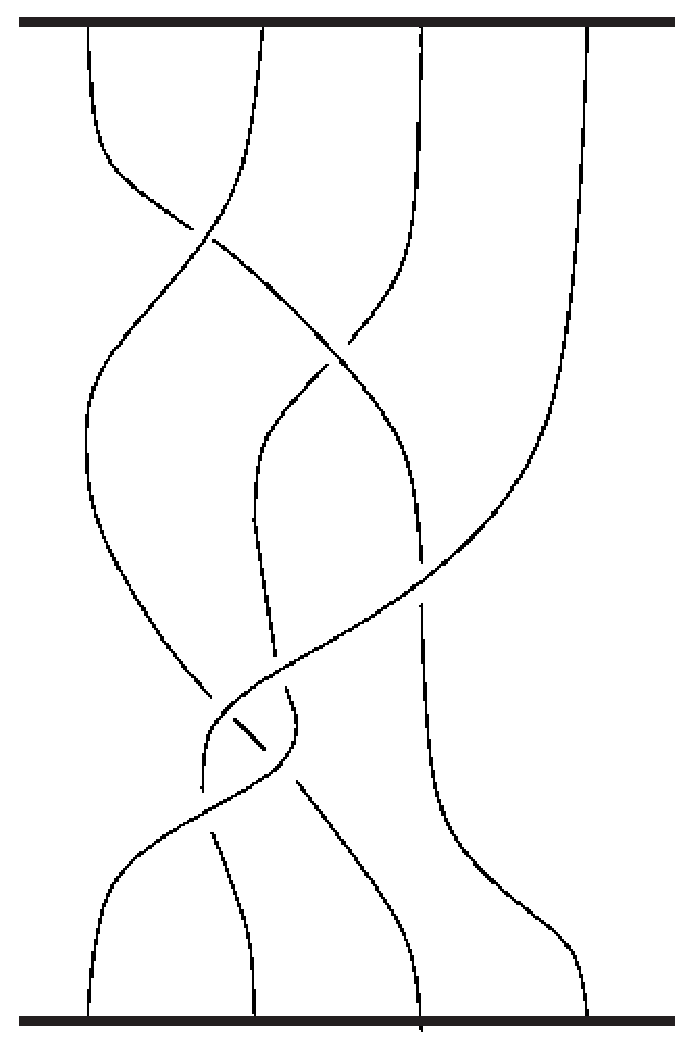
\includegraphics[angle=-90,width=4in]{4Braid.eps}
  \caption{This is an inserted EPS graphic}
  \label{fig:mygraph1}
\end{figure}
The graph in Figure \ref{fig:mygraph1} is from a PostScript file generated
by Maple and then converted to an Encapsulated Postcript File by the
{\tt ps2epsi} utility in ghostscript.

%The surface in Figure \ref{fig:mygraph2} was also generated by Maple.
%\begin{figure}[t]
% \centering
%  \includegraphics[angle=-90, width=4in]{myplot.epsi}  
%    \caption{This is another inserted EPS graphic}
%    \label{fig:mygraph2}
%\end{figure}
The figure is placed in the file {\tt graphics.tex} immediately after
the sentence ending ``also generated by Maple.''  Obviously it will not fit on 
the page with that sentence, so \LaTeX\ places the figure at the top
of the next page.  In the original version of the template,
the next page was the start of the list of bibliographic references.  
In order to get the list of references to
start on a fresh page,  we have had to add this text to the file.  The 
moral of the story is that typesetting decisions can have unintended
consequences. 
%This is the end of the file graphics.tex

